\documentclass[12pt, twoside]{article}
\usepackage[letterpaper, margin=0.25in, head=30pt, headsep=0.1in]{geometry}
\usepackage[english]{babel}
\usepackage[utf8]{inputenc}
\usepackage{amsmath}
\usepackage{amsfonts}
\usepackage{amssymb}
\usepackage{tikz}
\usetikzlibrary{quotes, angles}

\usepackage{graphicx}
\usepackage{enumitem}
\usepackage{multicol}

%\usepackage{pgfplots}
%\pgfplotsset{width=10cm,compat=1.9}
%\usepgfplotslibrary{statistics}
%\usepackage{pgfplotstable}
%\usepackage{tkz-fct}
%\usepackage{venndiagram}

\usepackage{fancyhdr}
\pagestyle{fancy}
\fancyhf{}
\renewcommand{\headrulewidth}{0pt} % disable the underline of the header
\raggedbottom
\newif\ifmeta
\metatrue %print standards and topics tags

\title{Math AI Worksheet Generator and Formative Assessment System}
\author{Chris Huson}
\date{October 2020}

%\fancyhead[RE]{\thepage}
%\fancyhead[RO]{\thepage \\ Name: \hspace{3cm}}
%\fancyhead[L]{BECA / Dr. Huson / 10th Grade Geometry\\* 7 June 2019}
%
%\begin{document}
%\subsubsection*{13.7 Homework: Cross sections, distance applications}
%\fancyhead[L]{BECA / Dr. Huson / Geometry 03-Volume+angle-bisectors\\* pset ID: 34}

\begin{document}

\subsubsection*{3.5 ReQuiz review, angle addition}
\begin{enumerate}

\item Demonstrate your ability to classify angles and use standard terminology.
\begin{enumerate}
  \item The given angle $\angle UVW$ is which of the following: acute, obtuse, or right?
  \begin{center}
    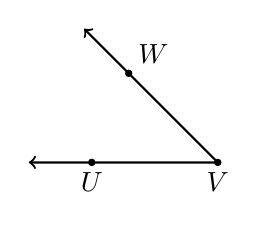
\begin{tikzpicture}[scale=.8]
      \draw  [<->, thick] (-3,0)--(0,0)--(135:3);
      \draw [fill] (-2,0) circle [radius=0.05] node[below]{$U$};
      \draw [fill] (0,0) circle [radius=0.05] node[below]{$V$};
      \draw [fill] (135:2) circle [radius=0.05] node[above right]{$W$};
    \end{tikzpicture}
  \end{center}
  \item Which of the following are true with respect to the angle, $m\angle PQR$?
  \begin{multicols}{2}
    True \hspace{0.25cm} False \hspace{0.25cm} It is an acute angle \\[0.5cm]
    True \hspace{0.25cm} False \hspace{0.25cm} It's measure is $90^\circ$\\[0.5cm]
    True \hspace{0.25cm} False \hspace{0.25cm} $\overrightarrow{QP} \perp \overrightarrow{QR}$ \\[0.5cm]
    \columnbreak
    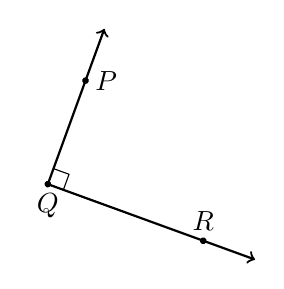
\begin{tikzpicture}[scale=0.7, rotate=-20]
      \draw [<->, thick] (4,0)--(0,0)--(0,3);
      \draw (0,0)++(0.3,0)--++(0,0.3)--+(-0.3,0);
      %\draw [fill] (-1,2.5) circle [radius=0.05] node[left ]{$B$};
      \draw [fill] (0,0) circle [radius=0.05] node[below]{$Q$};
      \draw [fill] (0,2) circle [radius=0.05] node[right]{$P$};
      \draw [fill] (3,0) circle [radius=0.05] node[above]{$R$};
    \end{tikzpicture}
  \end{multicols}
  \item What is sum of the degree measures of this linear pair, $\angle ABD$ and $\angle CBD$?
  \begin{center}
    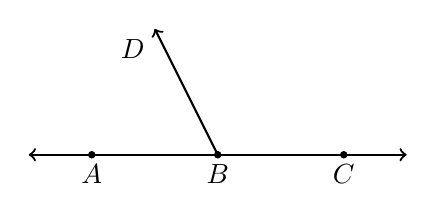
\begin{tikzpicture}[scale=.8, rotate=0]
      \draw  [<->, thick] (-3,0)--(3,0);
      \draw [->, thick] (0,0)--(-1, 2) node[below left]{$D$};
      \draw [fill] (-2,0) circle [radius=0.05] node[below]{$A$};
      \draw [fill] (0,0) circle [radius=0.05] node[below]{$B$};
      \draw [fill] (2,0) circle [radius=0.05] node[below]{$C$};
    \end{tikzpicture}
  \end{center}

  \end{enumerate}

\newpage
  \item As shown below, two lines intersect making four angles: $\angle 1$, $\angle 2$, $\angle 3$, and $\angle 4$.
  
    \begin{multicols}{2}  
      \begin{enumerate}
        \item Name a pair of vertical angles. \vspace{1.5cm}
        \item Given $m\angle 3 = 80^\circ$, write down $m\angle 1$. \vspace{1.5cm}
        \item Find $m\angle 4$. \vspace{2cm}
      \end{enumerate}
      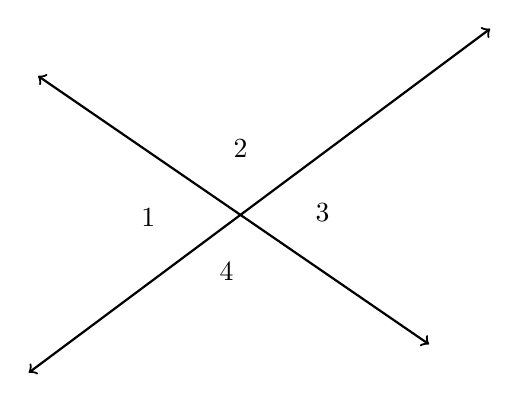
\begin{tikzpicture}[scale=0.7, rotate=20]
      \draw [<->, thick] (0,-1.5)--(10,1.5);
      \draw [<->, thick] (2,3.5)--(7,-3.5);
      \node at (3,.4){1};
      \node at (6,-.6){3};
      \node at (5,1){2};
      \node at (4,-1){4};
    \end{tikzpicture}
    \end{multicols}

\newpage
\subsubsection*{Angle addition situations}

\item Apply the Angle Addition postulate. Write and equation to support your work.
  \begin{multicols}{2}
    Given $m\angle CBD = 25^\circ$, $m\angle ABC = 90^\circ$. \\[0.5cm]
    Find $m \angle ABD$. \\
    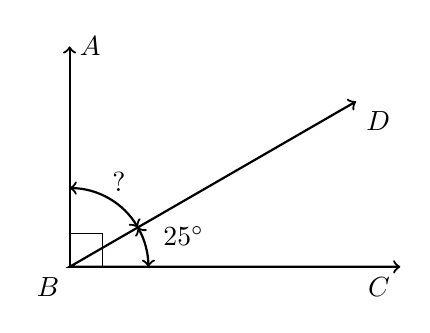
\begin{tikzpicture}[scale=1.4]
      \draw [<->, thick]
        (0:3) coordinate (a) node[below left] {$C$}
        -- (0,0) coordinate (b) node[below left] {$B$}
        -- (30:3) coordinate (c) node[below right] {$D$}
        pic["$25^\circ$", <->, draw=black, angle eccentricity=1.5, angle radius=1cm]
        {angle=a--b--c};
        \draw [<-, thick]
        (90:2) coordinate (d) node[right] {$A$}
        -- (0,0) coordinate (e)
        pic["$?$", <->, draw=black, angle eccentricity=1.25, angle radius=1cm]
        {angle=c--e--d};
      \draw (0,0)++(0.3,0)--++(0,0.3)--+(-0.3,0);
    \end{tikzpicture}
  \end{multicols}

\newpage
\item A linear pair is formed by two angles, $m\angle RUT = 2x+15$ and $m\angle SUT = 65^\circ$. \\[0.5cm] 
  Write an equation, then solve for $x$. \vspace{0.5cm}
    \begin{flushright}
      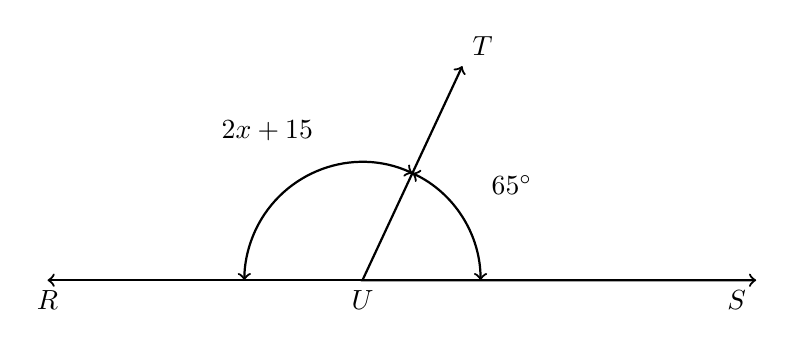
\begin{tikzpicture}[scale=1]
        \draw [<->, thick]
          (0:5) coordinate (a) node[below left] {$S$}
          -- (0,0) coordinate (b) node[below] {$U$}
          -- (65:3) coordinate (c) node[above right] {$T$}
          pic["$65^\circ$", <->, draw=black, angle eccentricity=1.5, angle radius=1.5cm]
          {angle=a--b--c};
          \draw [<-, thick]
          (180:4) coordinate (d) node[below] {$R$}
          -- (0,0) coordinate (e)
          pic["$2x+15$", <->, draw=black, angle eccentricity=1.5, angle radius=1.5cm]
          {angle=c--e--d};
          %\draw [->, thick] (0,0)--(-180:2) node[below right]{$A$};
          %\draw (0,0)++(-0.3,0)--++(0,0.3)--+(0.3,0);
      \end{tikzpicture}
    \end{flushright}
     
\newpage
\item Given $m\angle ABD = 2x+25$, $m\angle DBC = 4x$, and $m \angle ABC = 115^\circ$, as shown. \\[0.25cm]
  Model the situation with an equation, then solve for $x$. Check your solution for full credit.
  \begin{flushright}
      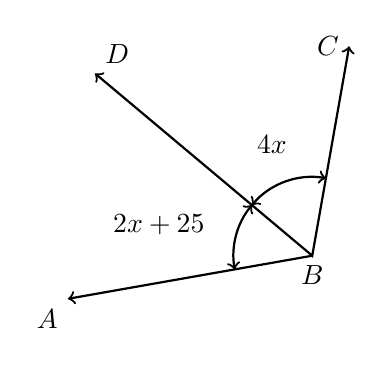
\begin{tikzpicture}[scale=1.8, rotate=90]
        \draw [<->, thick]
          (-10:1.5) coordinate (a) node[left] {$C$}
          -- (0,0) coordinate (b) node[below] {$B$}
          -- (50:2) coordinate (c) node[above right] {$D$}
          pic["$4x$", <->, draw=black, angle eccentricity=1.5, angle radius=1cm]
          {angle=a--b--c};
          \draw [<-, thick]
          (100:1.75) coordinate (d) node[below left] {$A$}
          -- (0,0) coordinate (e)
          pic["$2x+25 \hspace{1cm}$", <->, draw=black, angle eccentricity=1.5, angle radius=1cm]
          {angle=c--e--d};
      \end{tikzpicture}
    \end{flushright}

\newpage
\item Given vertical angles, $m\angle APD = 6x-8$, $m\angle BPC = 5x+5$, as shown. \\[0.25cm]
  Find $x$. Check your solution for full credit.
  \begin{flushright}
      \begin{tikzpicture}[scale=1.8, rotate=0]
        \draw [<->, thick]
          (0:2) coordinate (a) node[below left] {$C$}
          -- (0,0) coordinate (b) node[below right] {$P$}
          -- (70:1.5) coordinate (c) node[below right] {$B$}
          pic["$5x+5$", <->, draw=black, angle eccentricity=1.75, angle radius=1cm]
          {angle=a--b--c};
          \draw [<->, thick]
          (180:2) coordinate (d) node[above right] {$A$}
          -- (0,0) coordinate (e)
          -- (250:2) coordinate (f) node[above left] {$D$}
          pic["$6x-8$", <->, draw=black, angle eccentricity=1.75, angle radius=1cm]
          {angle=d--e--f};
      \end{tikzpicture}
    \end{flushright}
 
\newpage
\item In the diagram shown, $\overrightarrow{BD} \perp \overleftrightarrow{ABC}$ with angle measures marked. 
  Find $x$. \\[0.25cm] 
  Show the check for full credit.\vspace{0.25cm}
    \begin{multicols}{2}
      $m\angle DBE = 6x-16^\circ$ \\[0.25cm]
      $m\angle EBC = 3x+7^\circ$ \\[0.25cm]
      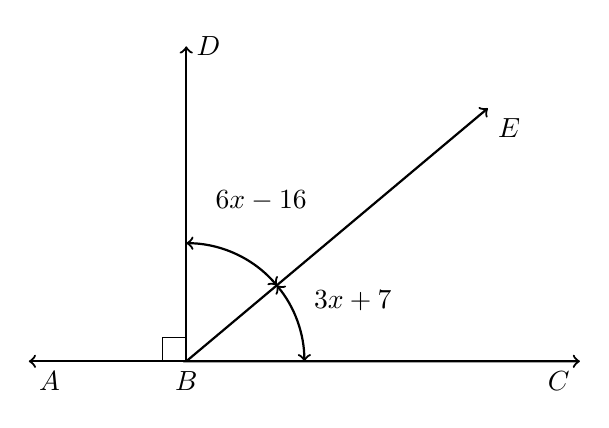
\begin{tikzpicture}[scale=1]
        \draw [<->, thick]
          (0:5) coordinate (a) node[below left] {$C$}
          -- (0,0) coordinate (b) node[below] {$B$}
          -- (40:5) coordinate (c) node[below right] {$E$}
          pic["$3x+7$", <->, draw=black, angle eccentricity=1.5, angle radius=1.5cm]
          {angle=a--b--c};
          \draw [<-, thick]
          (90:4) coordinate (d) node[right] {$D$}
          -- (0,0) coordinate (e)
          pic["$6x-16$", <->, draw=black, angle eccentricity=1.5, angle radius=1.5cm]
          {angle=c--e--d};
          \draw [->, thick] (0,0)--(-180:2) node[below right]{$A$};
          \draw (0,0)++(-0.3,0)--++(0,0.3)--+(0.3,0);
      \end{tikzpicture}
    \end{multicols}

\newpage
\item Spicy: Given $\overleftrightarrow{ABC}$, right angle $\angle DBE$, $m\angle ABE = 4x+4$, and $m\angle CBD = 2x+2$. \\[0.5cm] 
  Find $m\angle CBD$. \vspace{0.5cm}
    \begin{flushright}
      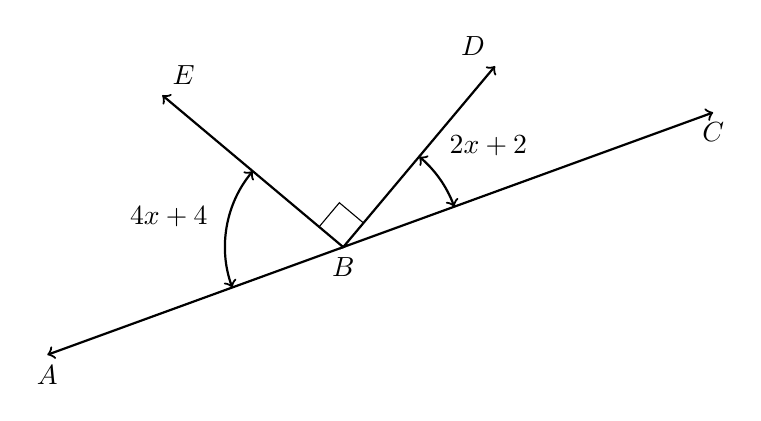
\begin{tikzpicture}[scale=1, rotate=50]
        \draw [<->, thick]
          (-30:5) coordinate (a) node[below] {$C$}
          -- (0,0) coordinate (b) node[below] {$B$}
          -- (3,0) coordinate (c) node[above left] {$D$}
          pic["$2x+2$", <->, draw=black, angle eccentricity=1.5, angle radius=1.5cm]
          {angle=a--b--c};
          \draw [<->, thick]
          (150:4) coordinate (d) node[below] {$A$}
          -- (0,0) -- (0, 3) coordinate (e) node[above right] {$E$}
          pic["$4x+4$", <->, draw=black, angle eccentricity=1.5, angle radius=1.5cm]
          {angle=e--b--d};
          \draw (0,0)++(0.4,0)--++(0,0.4)--+(-0.4,0);
      \end{tikzpicture}
    \end{flushright}

\newpage
\item Spicy: Ray $\overrightarrow{BF}$ is the angle bisector of $\angle ABC$. Given that the angle measures are $m\angle ABF = 7x-5$ and $m\angle CBF = 5x+13$. \\[0.5cm] 
  Find $m\angle ABC$. \vspace{0.5cm}
    \begin{flushright}
      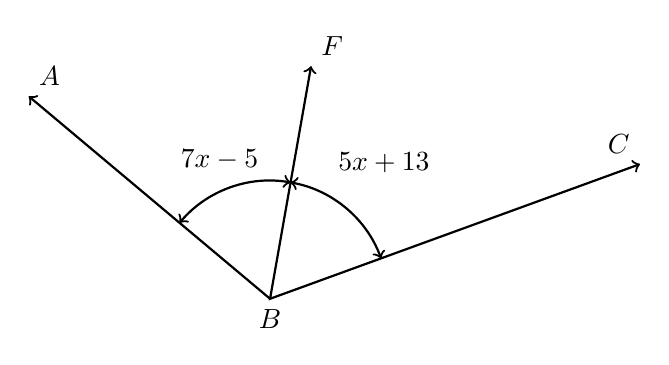
\begin{tikzpicture}[scale=1, rotate=20]
        \draw [<->, thick]
          (0:5) coordinate (a) node[above left] {$C$}
          -- (0,0) coordinate (b) node[below] {$B$}
          -- (60:3) coordinate (c) node[above right] {$F$}
          pic["$5x+13$", <->, draw=black, angle eccentricity=1.5, angle radius=1.5cm]
          {angle=a--b--c};
          \draw [<-, thick]
          (120:4) coordinate (d) node[above right] {$A$}
          -- (0,0) coordinate (e)
          pic["$7x-5$", <->, draw=black, angle eccentricity=1.25, angle radius=1.5cm]
          {angle=c--e--d};
          %\draw [->, thick] (0,0)--(-180:2) node[below right]{$A$};
          %\draw (0,0)++(-0.3,0)--++(0,0.3)--+(0.3,0);
      \end{tikzpicture}
    \end{flushright}

\end{enumerate}
\end{document}